% We now present Snooze~\cite{feller:ccgrid12} as a second case study of how
% to implement and simulate advanced algorithms.
% We present its architecture summarizing its main
% characteristics from its original presentation~\cite{feller:ccgrid12} and
% additional information  stemming from personal communications of the Snooze
% developers and its implementation~\cite{snoozeweb,snoozedev14}.

% \subsubsection{Architecture}
% \label{sec:snoozeArchi}

Snooze~\cite{snoozeweb,snoozedev14} harnesses a hierarchical
architecture in order to support load balancing and fault tolerance,
cf.\ Fig.~\ref{fig:snoozearch}. At the top of the hierarchy, a
\emph{group leader (GL)} centralizes information about the whole
cluster using summary data about \emph{group managers (GMs)} that
constitute the intermediate layer of the hierarchy. GMs manage a
number of \emph{local controllers (LCs)} that, in turn, manage the VMs
assigned to nodes.
% The GL and the GMs are deployed on service nodes while the LCs are
% executed on hosting node.

\begin{wrapfigure}{r}{.4\linewidth}
  {\centering ~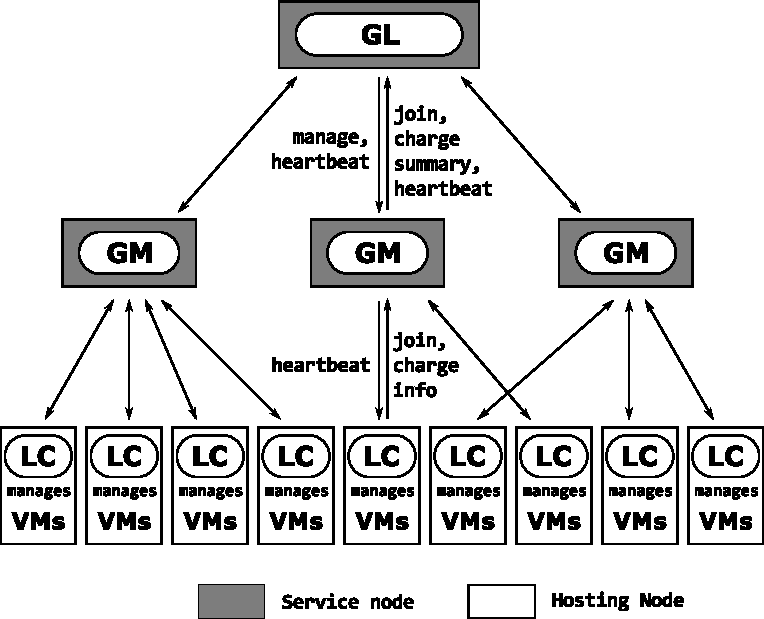
\includegraphics[width=.99\linewidth]{figures/snoozearch.pdf}}
  \caption{Snooze Architecture Overview}
  \label{fig:snoozearch}
\end{wrapfigure}
During execution, higher-level components periodically send heartbeats
to lower-level ones; monitoring information, \eg about the system
load, is also sent periodically in the opposite direction. In order to
propagate information, Snooze relies on hardware support for multicast
communication. Finally, a number of replicated entry points allows
clients to contact the GL, \eg in order to submit new VMs for
integration into the system.

\emph{Simulation using \vmps.~} The \texttt{XHOST}, \texttt{XVM} and
\texttt{SimulatorManager} classes have been harnessed to implement the
core architectural abstractions (\ie VM monitoring and manipulations),
the remaining concepts and algorithms of Snooze have been implemented
using Simgrid's primitives and standard Java mechanisms.
%
Communication between Snooze actors is implemented based on Simgrid's
primitives for, mainly asynchronous, event handling.
Hardware\-sup\-ported multicast communication that is used, \eg
to relay heartbeats, is implemented as a dedicated actor that manages
a state representing GL and GM heartbeat groups and relaying heartbeat
events.
%
Finally, our Snooze simulation uses, as its original counterpart, a
multi-threaded implementation (\ie based on multiple SG processes) in
order to optimize reactivity even for large groups of LCs (or GMs)
that have to be managed by one GM (or GL).

% \subsubsection{Algorithms}
% \label{sec:snoozeAlgs}

% Apart from the handling of faults (described below), two types of
% algorithms are of major importance for the administration of the
% Snooze architecture: the algorithms that enable components to
% dynamically enter the system and the algorithms that propagate info
% between the components.

% A GL is created, if it does not exist, by promotion of a GM that is
% selected according to some leader election algorithm. When a GM joins
% a cluster, it starts listening on a predefined channel for the
% heartbeat of the GL and registers once it has received the
% heartbeat. New LCs first also wait for the GL heartbeat, contact the
% GL then in order to obtain a GM assignment, and finally register at
% the GM assigned to them.

% Two kinds of (load) information are passed within the system: the
% periodic heartbeat message sent by the GL and the GMs; second,
% periodic load information sent from LCs to their respective GMs and
% summary load info sent by the GMs to the GL.

% \subsubsection{Fault tolerance}

% GLs, GMs and LCs may fail during the system execution. System
% components identify that a node on the corresponding higher-level node
% has failed (the GL in case of a GM, a GM in the case of an LC) in an
% asynchronous fashion through the lack of heartbeat messages.

% In the case of a GL failure, one of the GMs becomes the new GL, stops
% its GM activities and prevents the LCs it manages so that they can
% start rejoining the system. If a GM fails, the GL and the LCs it has
% managed will become aware of it based on the lack of heartbeats,
% update its data structures and, for the LCs, rejoin the system. If an
% LC fails, its GM will finally learn of it due to the missing heartbeat
% and charge information of the LC. The GM will then remove the LC from
% its data structures.


% \subsubsection{Variants}
% \label{sec:snoozeVariants}

% Our simulation framework facilitates the simulation of variants of
% placement algorithms. In the following, we present three non-trivial
% variants that we have implemented and explored: a variant of the
% assignment algorithm of LCs to GMs, periodic vs.\ reactive scheduling,
% and a variant of the algorithms of how GMs and LCs join the system.


% \paragraph{Assignment of LCs to GMs}

% LCs are assigned to GMs by the GL as part of the LC join protocol. In
% Snooze's native implementation LCs are assigned in a round-robin
% fashion to the known GMs. If GMs join (and leave) the system at the
% same time as LCs, a round-robin strategy at join time, however, does
% not ensure an even distribution. This may happen, for instance at
% startup time of the system, when new GMs and LCs enter the system, or
% in case of failures, which trigger GM and LC joins. In order to
% evaluate the imbalance resulting from a round-robin strategy (as well
% as others) we have implemented the LC assignment protocol in a modular
% fashion and applied it in diverse highly-dynamic settings in which GMs
% and LCs enter the system at the same time. Furthermore, we have
% implemented a best-fit strategy that assigns LCs to GMs with minimal
% load or to GMs with the smallest number of assigned LCs (if several
% GMs with minimal load exist). The best-fit strategy can significantly
% improve the scheduling characteristics of hierarchical placement
% algorithms as shown by the experimental data presented in
% Sec.~\ref{sec:snoozeVariantsEval}. Furthermore, it should always be
% at least as good as the round-robin strategy (the corresponding proof
% is left to future work).


% \paragraph{Periodic vs.\ reactive scheduling}

% Snooze~\cite{feller:ccgrid12} schedules VMs in a periodic fashion:
% after a fixed time period a GM calls the scheduler in order to resolve
% resource conflicts among the LCs it manages. The information whether a
% resource conflict has to be handled is taken based on the summary
% information that is periodically sent by the LCs to the GM.

% We have provided an alternative, reactive, strategy to scheduling: as
% soon as they occur, LCs avert their GMs of resource conflicts; the GMs
% then initiate scheduling. Implementing this reactive scheme can be
% done using our framework in two manners: either by implementing
% additional asynchronous transmissions as a real implementation of the
% necessary state updates would proceed or, in a much more lightweight
% manner, through direct accesses by the GMs to the states of their
% respective LCs. While the latter does not mimic a real implementation
% closely, it can be harnessed to yield a valid simulation: delays
% induced by communication in the ``real'' implementation, for instance,
% can be easily added as part of the lightweight simulation. We have
% implemented this lightweight variant of reactive scheduling.


% \paragraph{Variants of the join algorithms}

% The join algorithms, see Sec.~\ref{sec:snoozeAlgs}, are crucial to the
% correctness of Snooze for two main reasons: (i) they have to be
% efficient because they can easily form a bottleneck if large numbers
% of LCs (GMs) have to be registered at a GM (LC); (ii) they are
% multi-phase protocols whose correctness especially in the presence of
% faults is difficult to ensure.

% In order to investigate the corresponding trade-offs, we have used our
% framework to implement join algorithms that may be interrupted at any
% time, repeat the the on-going phase a number of times before
% reinitiating, if necessary, the entire protocol. Furthermore, the join
% protocol is parameterized, \eg, in the number of threads used to
% handle registration requests.

% Finally, our framework has enabled us to test another aspect of
% Snooze's join algorithm as presented by
% Feller~\etal.~\cite{feller:ccgrid12},
% \MS[MS]{If we succeed to perform the experiment comparing both
%   approach, this paragraph should be highlighted.}
% a strategy we call the GM rejoin
% strategy (GRJ): all GMs should rejoin if a new GM enters the
% system. While GRJ supports a form of load balancing (because all LCs
% are reassigned to the new set of GMs), our simulation has shown that
% this strategy significantly increases the time necessary for
% registering GMs and LCs compared to a simpler strategy that does not
% modify existing GMs in case a new GM enters the system. This handicap
% is particularly pronounced if joins of GMs may be interrupted due to
% faults. Concretely, experiments involving 20 GMs and 200 LCs have
% shown that this strategy often multiplies the time necessary to join
% all 220 components by 10 or more compared to the simple join
% strategy. While the qualitative result that the more complex strategy
% presented in the paper results in a more time-consuming join process
% is not very surprising, the extent of the resulting degradation was
% surprising.



%%% Local Variables:
%%% mode: latex
%%% TeX-master: "main"
%%% End:
